\documentclass[onecolumn]{article}
%\usepackage{url}
%\usepackage{algorithmic}
\usepackage[a4paper]{geometry}
\usepackage{datetime}
\usepackage[margin=2em, font=small,labelfont=it]{caption}
\usepackage{graphicx}
\usepackage{mathpazo} % use palatino
\usepackage[scaled]{helvet} % helvetica
\usepackage{microtype}
\usepackage{amsmath}
\usepackage{subfigure}
\usepackage{hyperref}
\usepackage{graphicx}
\makeatletter


\usepackage{listings} 
\usepackage{color}
\definecolor{dkgreen}{rgb}{0,0.6,0}
\definecolor{gray}{rgb}{0.5,0.5,0.5}
\definecolor{mauve}{rgb}{0.58,0,0.82}


\hypersetup{   
    colorlinks=true,
    linkcolor=blue,
    filecolor=magenta,
    urlcolor=blue,
    pdftitle={Overleaf Example},
    pdfpagemode=FullScreen,
}

\lstset{frame=tb,
  language=python,
  aboveskip=3mm,
  belowskip=3mm,
  showstringspaces=false,
  columns=flexible,
  basicstyle={\small\ttfamily},
  numbers=none,
  numberstyle=\tiny\color{gray},
  keywordstyle=\color{blue},
  commentstyle=\color{dkgreen},
  stringstyle=\color{mauve},
  breaklines=true,
  breakatwhitespace=true,
  tabsize=2
}

\documentclass[12pt]{article}
\usepackage[many]{tcolorbox}
\usepackage{marginnote}
\usepackage{kantlipsum}
\tcbuselibrary{skins,breakable}
\newtcolorbox{story}[1][]{
    width=\textwidth,
    colback=magenta!20,
    colframe=red!75!black,
    colbacktitle=blue!75!black,
    fonttitle=\bfseries,
    left=0ex,
    right=0ex,
    top=0pt,
    arc=0pt,
    outer arc=0pt,
    leftrule=0pt,
    rightrule=0pt,
    toprule=0pt,
    bottomrule=0pt,
    breakable,
    enhanced jigsaw,
    title= #1}




% Letterspacing macros
\newcommand{\spacecaps}[1]{\textls[200]{\MakeUppercase{#1}}}
\newcommand{\spacesc}[1]{\textls[50]{\textsc{\MakeLowercase{#1}}}}

\title{Hadoop Deployment}


\begin{document}

\maketitle

\tableofcontents

\section{Preinstall}


\subsection{ssh connection}

\textbf{pdsh} can run multiple remote commands in parallel. 

\begin{lstlisting}[language=Python, caption= Install SSH and PDSH]
sudo apt install ssh
\end{lstlisting}

\begin{figure}[ht!]
\centering
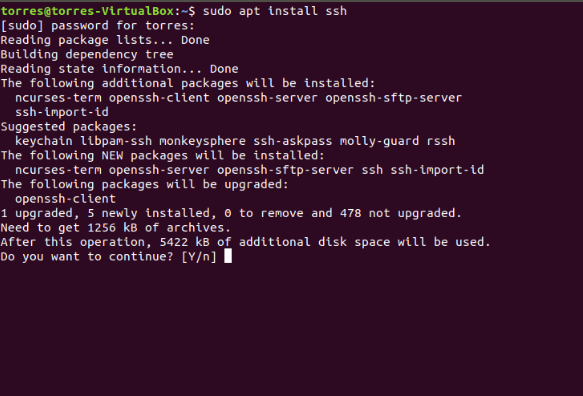
\includegraphics[width=8cm]{1.png}
\caption{\label{}}
\end{figure}

\begin{lstlisting}[language=Python, caption= Install SSH and PDSH]
sudo apt install pdsh
\end{lstlisting}

\begin{figure}[ht!]
\centering
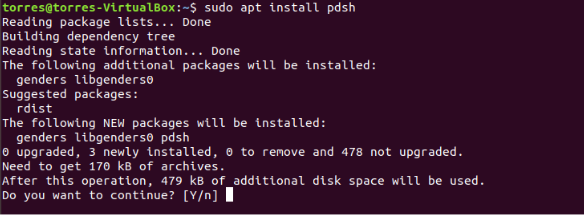
\includegraphics[width=8cm]{2.png}
\caption{\label{}}
\end{figure}

\begin{lstlisting}[language=Python, caption= Install PDSH]
nano .bashrc
\end{lstlisting}

At the end of the file just write the following line:
\begin{lstlisting}[language=Python, caption= ]
export PDSH_RCMD_TYPE=ssh
\end{lstlisting}

\begin{figure}[ht!]
\centering
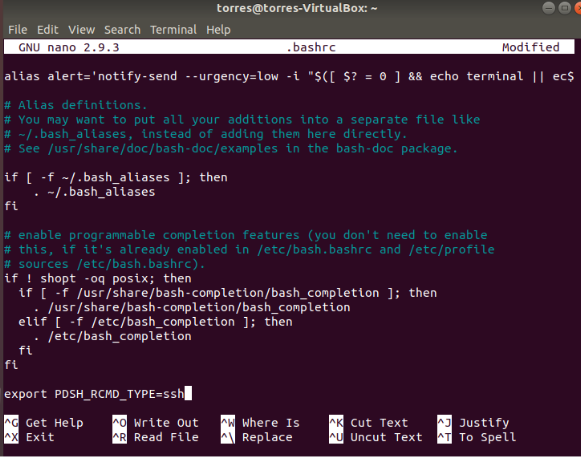
\includegraphics[width=8cm]{3.png}
\caption{\label{}}
\end{figure}


Now let’s configure SSH. Let’s create a new key using the following command:

\begin{lstlisting}[language=Python, caption= ssh-keygen]
ssh-keygen -t rsa -P ""
\end{lstlisting}

\begin{figure}[ht!]
\centering
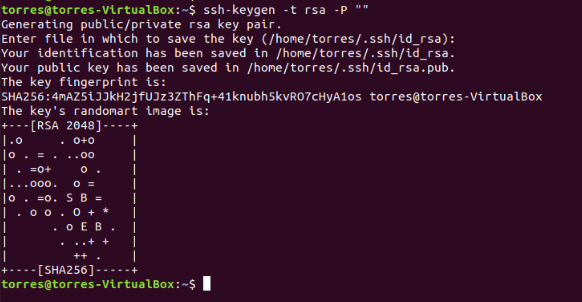
\includegraphics[width=8cm]{4.png}
\caption{\label{}}
\end{figure}


\begin{lstlisting}[language=Python, caption= ssh-keygen]
cat ~/.ssh/id_rsa.pub >> ~/.ssh/authorized_keys
\end{lstlisting}

\begin{figure}[ht!]
\centering

\includegraphics[width=8cm]{5.png}
\caption{\label{}}
\end{figure}



Now we can verify the SSH configuration by connecting to the localhost:

\begin{lstlisting}[language=Python, caption= ssh local host]
ssh localhost
\end{lstlisting}

\begin{figure}[ht!]
\centering
\includegraphics[width=8cm]{localhost.png}
\caption{\label{}}
\end{figure}

\subsection{java installation}

Install OpenJDK, the default Java Development Kit
\begin{lstlisting}[language=Python, caption= jdk]
sudo apt install default-jdk
\end{lstlisting}



This step isn’t really a step, it’s just to check if Java is now correctly installed:

\begin{lstlisting}[language=Python, caption= version check]
java -version
\end{lstlisting}

\begin{figure}[ht!]
\centering
\includegraphics[width=8cm]{java_version.png}
\caption{\label{}}
\end{figure}


\section{Installing Hadoop}

\subsection{hadoop version}
In example I used the hadoop-3.0.3 version but we can use any version that we want to change the version in this link:

\url{https://archive.apache.org/dist/hadoop/core/hadoop-3.0.3/} 

\subsection{download hadoop}

Download Hadoop using the following command:

\begin{lstlisting}[language=Python, caption= version check]
sudo wget https://archive.apache.org/dist/hadoop/core/hadoop-3.0.3/hadoop-3.0.3.tar.gz
\end{lstlisting}


\begin{lstlisting}[language=Python, caption= version check]
sudo wget https://archive.apache.org/dist/hadoop/core/hadoop-3.0.3/hadoop-3.0.3.tar.gz.mds
\end{lstlisting}

\begin{figure}[ht!]
\centering
\includegraphics[width=8cm]{tar.png}
\caption{\label{}}
\end{figure}

Then run the verification:

\begin{lstlisting}[language=Python, caption= version check]
shasum -a 256 hadoop-3.0.3.tar.gz
\end{lstlisting}

Compare this value with the SHA-256 value in the .mds file:

\begin{lstlisting}[language=Python, caption= version check]
cat hadoop-3.0.3.tar.gz.mds
\end{lstlisting}


\begin{figure}[ht!]
\centering
\includegraphics[width=8cm]{sha.png}
\caption{\label{}}
\end{figure}

\subsection{extract hadoop tar}

Now that we’ve verified that the file wasn’t corrupted or changed, we’ll use the tar command with the \textbf{-x} flag to extract, \textbf{-z} to uncompress, \textbf{-v} for verbose output, and \textbf{-f} to specify that we’re extracting from a file. Use tab-completion or substitute the correct version number in the command below:

\begin{lstlisting}[language=Python, caption= Output]
tar -xzvf hadoop-3.0.3.tar.gz
\end{lstlisting}

\begin{figure}[ht!]
\centering
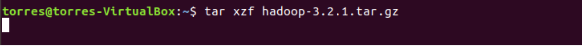
\includegraphics[width=8cm]{10.png}
\caption{\label{}}
\end{figure}

Finally, we’ll move the extracted files into /usr/local, the appropriate place for locally installed software. Change the version number, if needed, to match the version you downloaded.

\subsection{move extracted file}

\begin{lstlisting}[language=Python, caption= Move]
sudo mv hadoop-3.0.3 /usr/local/hadoop
\end{lstlisting}

\begin{figure}[ht!]
\centering
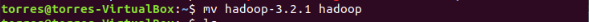
\includegraphics[width=8cm]{11.png}
\caption{\label{}}
\end{figure}

\section{Configuring Hadoop’s Java Home}

The path to Java, \textbf{/usr/bin/java} is a symlink to \textbf{/etc/alternatives/java}, which is in turn a symlink to default Java binary. We will use \textbf{readlink} with the -f flag to follow every symlink in every part of the path, recursively. Then, we’ll use sed to trim bin/java from the output to give us the correct value for JAVA HOME.\\

To find the default Java path:
\begin{lstlisting}[language=Python, caption= java path]
readlink -f /usr/bin/java | sed "s:bin/java::"
\end{lstlisting}



We can copy this output to set Hadoop’s Java home to this specific version, which ensures that if the default Java changes, this value will not.\\\\

To begin, open \textbf{hadoop-env.sh}:

\begin{lstlisting}[language=Python, caption= java path]
sudo nano /usr/local/hadoop/etc/hadoop/hadoop-env.sh
\end{lstlisting}

\subsection{option 1: set a static value}

\begin{lstlisting}[language=Python, caption= /usr/local/hadoop/etc/hadoop/hadoop-env.sh]
 . . .
#export JAVA_HOME=${JAVA_HOME}
export JAVA_HOME=/usr/lib/jvm/java-11-openjdk-amd64/
 . . . 
\end{lstlisting}

\subsection{option 2: use readlink to set the value dynamically}

It is prefered setting dynamically.\\\\

\begin{lstlisting}[language=Python, caption= /usr/local/hadoop/etc/hadoop/hadoop-env.sh]
 . . .
#export JAVA_HOME=${JAVA_HOME}
export JAVA_HOME=$(readlink -f /usr/bin/java | sed "s:bin/java::")
 . . . 
\end{lstlisting}

\begin{figure}[ht!]
\centering
\includegraphics[width=12cm]{java_home.png}
\caption{\label{}}
\end{figure}

\subsection{set the value on environment}

Open the environment file on nano with this command:

\begin{lstlisting}[language=Python, caption=  s]
sudo nano /etc/environment
\end{lstlisting}


Then, add the following configurations: (\textbf{Path is in one line} )

\begin{lstlisting}[language=Python, caption= sudo nano /etc/environment ]
PATH=
"/usr/local/sbin:/usr/local/bin:/usr/sbin:/usr/bin:/sbin:/bin:/usr/games:/usr/
local/games:/usr/local/hadoop/bin:/usr/local/hadoop/sbin"
JAVA_HOME=$(readlink -f /usr/bin/java | sed "s:bin/java::")
\end{lstlisting}


\section{Create Hadoop User}

we will add a user called \textbf{hadoopuser}, and we will set up it’s configurations:

\begin{lstlisting}[language=Python, caption= sudo nano /etc/environment ]
sudo adduser hadoopuser
\end{lstlisting}

Provide the password and you can leave the rest blank, just press Enter.

\begin{figure}[ht!]
\centering
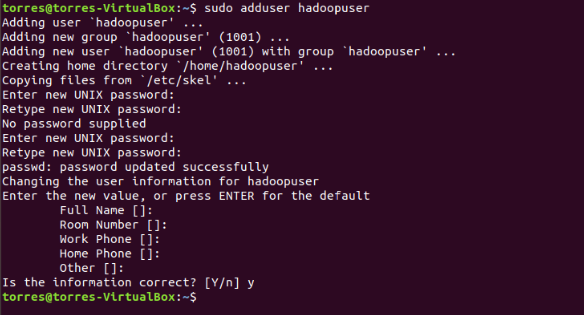
\includegraphics[width=6cm]{14.png}
\caption{\label{}}
\end{figure}
.\\\\\\\\\\\\\\\\
Now type these commands :

\begin{lstlisting}[language=Python, caption= a ]
sudo usermod -aG hadoopuser hadoopuser
sudo chown hadoopuser:root -R /usr/local/hadoop/
sudo chmod g+rwx -R /usr/local/hadoop/
sudo adduser hadoopuser sudo
\end{lstlisting}

\begin{figure}[ht!]
\centering
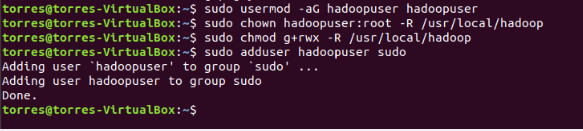
\includegraphics[width=6cm]{15.png}
\caption{\label{}}
\end{figure}

\subsection{check your ip address}

\begin{lstlisting}[language=Python, caption= a ]
ip addr
\end{lstlisting}

\begin{figure}[ht!]
\centering
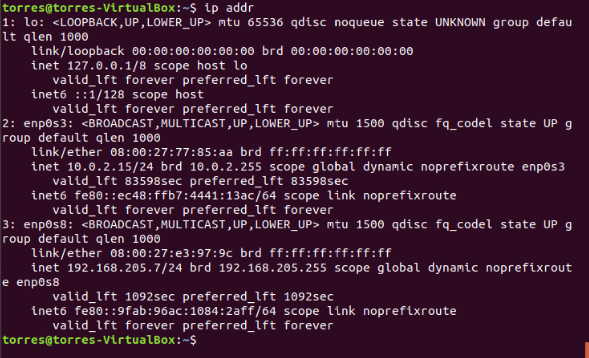
\includegraphics[width=8cm]{17.png}
\caption{\label{}}
\end{figure}

Open the hosts file and insert your Network configurations:

\begin{lstlisting}[language=Python, caption= a ]
sudo nano /etc/hosts
\end{lstlisting}

\begin{figure}[ht!]
\centering
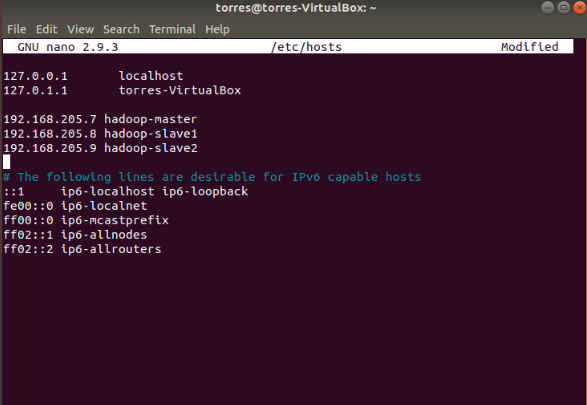
\includegraphics[width=8cm]{18.png}
\caption{\label{}}
\end{figure}

On the master , open the hostname file on nano:

\begin{lstlisting}[language=Python, caption= a ]
sudo nano /etc/hostname
\end{lstlisting}

\begin{figure}[ht!]
\centering
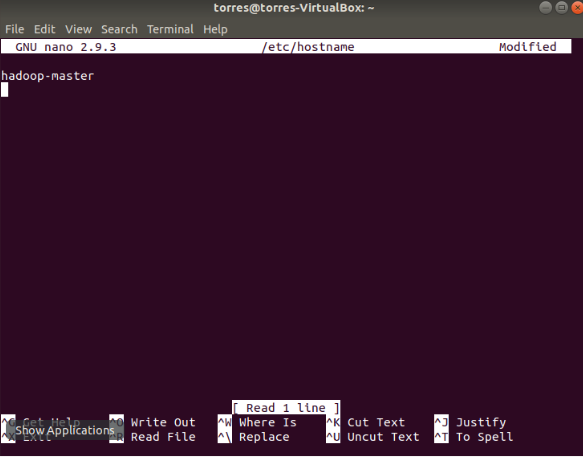
\includegraphics[width=8cm]{19.png}
\caption{\label{}}
\end{figure}
You should do the :same for slave nodes:

\begin{figure}[ht!]
\centering
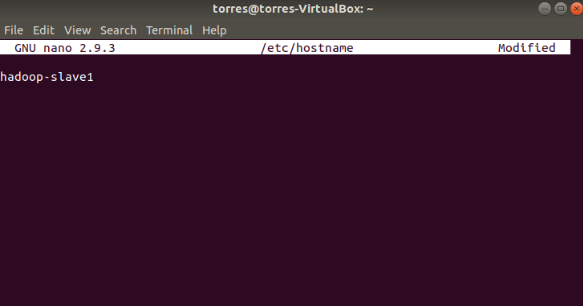
\includegraphics[width=8cm]{20.png}
\caption{\label{}}
\end{figure}

\begin{figure}[ht!]
\centering
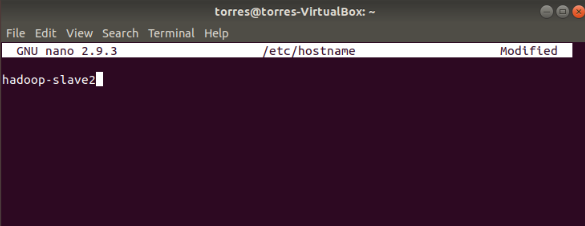
\includegraphics[width=8cm]{21.png}
\caption{\label{}}
\end{figure}

:\\\\\\

Also, you should reboot all of them so this configuration taked effect:

\begin{lstlisting}[language=Python, caption= a ]
sudo reboot
\end{lstlisting}

\section{On Hadoop User}

Configure the SSH on hadoop-master, with the hadoopuser. This is the command:

\begin{lstlisting}[language=Python, caption= a ]
su - hadoopuser
\end{lstlisting}

\begin{figure}[ht!]
\centering
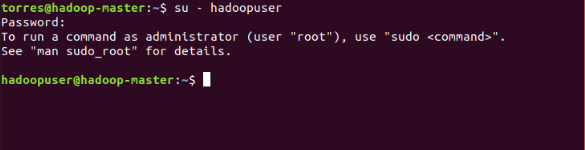
\includegraphics[width=8cm]{22.png}
\caption{\label{}}
\end{figure}

\subsection{ssh}

Create an SSH key:

\begin{lstlisting}[language=Python, caption= a ]
ssh-keygen -t rsa
\end{lstlisting}

\begin{figure}[ht!]
\centering
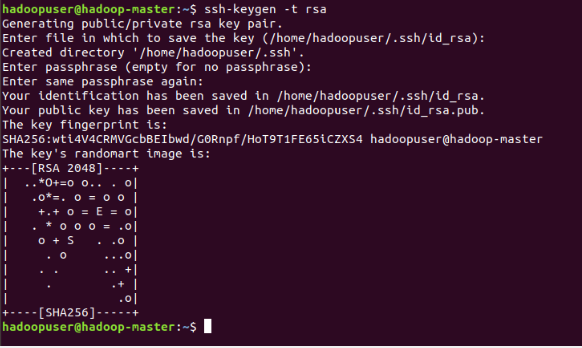
\includegraphics[width=8cm]{23.png}
\caption{\label{}}
\end{figure}

Now we need to copy the SSH key to all the users. Use this command:

\begin{lstlisting}[language=Python, caption= a ]
ssh-copy-id hadoopuser@hadoop-master
\end{lstlisting}

\begin{figure}[ht!]
\centering
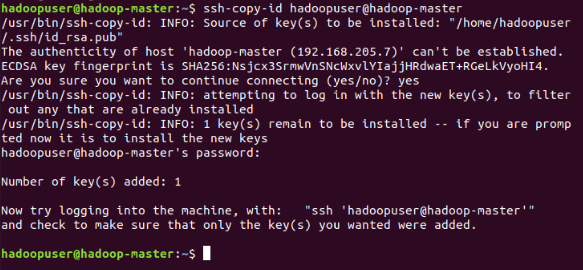
\includegraphics[width=8cm]{24.png}
\caption{\label{}}
\end{figure}

\begin{lstlisting}[language=Python, caption= a ]
ssh-copy-id hadoopuser@hadoop-slave1
\end{lstlisting}

\begin{figure}[ht!]
\centering
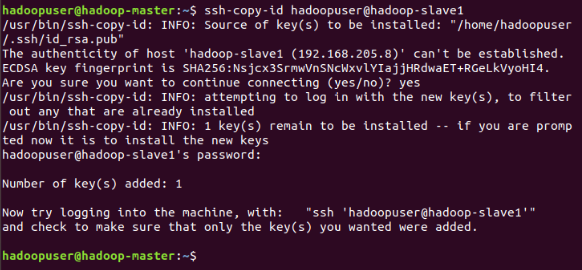
\includegraphics[width=8cm]{25.png}
\caption{\label{}}
\end{figure}

\begin{lstlisting}[language=Python, caption= a ]
ssh-copy-id hadoopuser@hadoop-slave2
\end{lstlisting}

\begin{figure}[ht!]
\centering
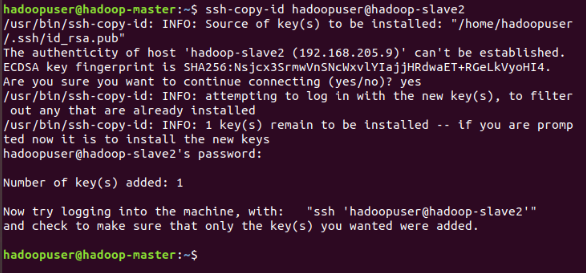
\includegraphics[width=8cm]{26.png}
\caption{\label{}}
\end{figure}

\section{Add Hadoop Services}

\subsection{core-site.xml}

On hadoop-master, open core-site.xml file on nano:

\begin{lstlisting}[language=Python, caption= a ]
sudo nano /usr/local/hadoop/etc/hadoop/core-site.xml
\end{lstlisting}

\begin{figure}[ht!]
\centering
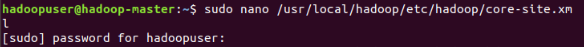
\includegraphics[width=8cm]{27.png}
\caption{\label{}}
\end{figure}


Then add the following configurations:

\begin{lstlisting}[language=Python, caption= a ]
<configuration>
<property>
<name>fs.defaultFS</name>
<value>hdfs://hadoop-master:9000</value>
</property>
</configuration>
\end{lstlisting}

\begin{figure}[ht!]
\centering
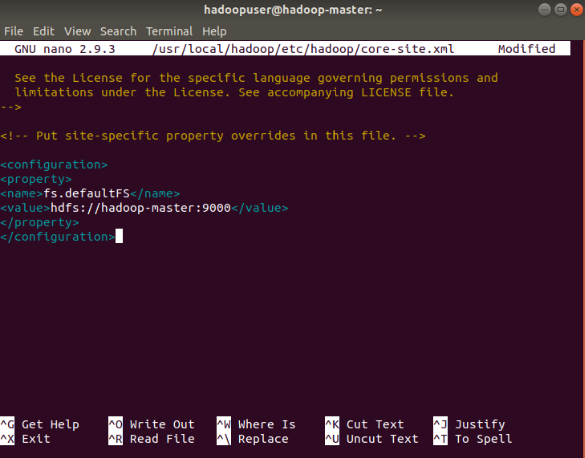
\includegraphics[width=8cm]{28.png}
\caption{\label{}}
\end{figure}

\subsection{hdfs-site.xml}

Still on hadoop-master, open the hdfs-site.xml file.

\begin{lstlisting}[language=Python, caption= a ]
sudo nano /usr/local/hadoop/etc/hadoop/hdfs-site.xml
\end{lstlisting}

\begin{figure}[ht!]
\centering
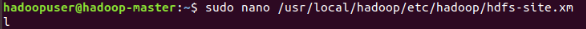
\includegraphics[width=8cm]{29.png}
\caption{\label{}}
\end{figure}


Add the following configurations:

\begin{lstlisting}[language=Python, caption= a ]
<configuration>
<property>
<name>dfs.namenode.name.dir</name><value>/usr/local/hadoop/data/nameNode</value>
</property>
<property>
<name>dfs.datanode.data.dir</name><value>/usr/local/hadoop/data/dataNode</value>
</property>
<property>
<name>dfs.replication</name>
<value>2</value>
</property>
</configuration>
\end{lstlisting}

\begin{figure}[ht!]
\centering
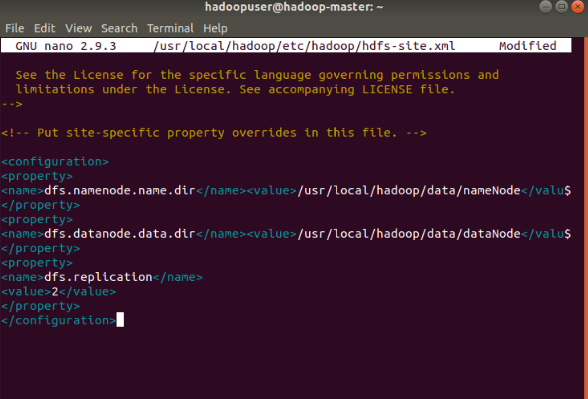
\includegraphics[width=8cm]{30.png}
\caption{\label{}}
\end{figure}
.\\\\
\subsection{copy to workers}

We’re still on hadoop-master, let’s open the workers file:

\begin{lstlisting}[language=Python, caption= a ]
sudo nano /usr/local/hadoop/etc/hadoop/workers
\end{lstlisting}

\begin{figure}[ht!]
\centering
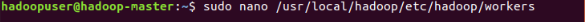
\includegraphics[width=8cm]{31.png}
\caption{\label{}}
\end{figure}





Add these two lines: (the slave names, remember the hosts file?)

\begin{lstlisting}[language=Python, caption= a ]
hadoop-slave1
hadoop-slave2
\end{lstlisting}

\begin{figure}[ht!]
\centering
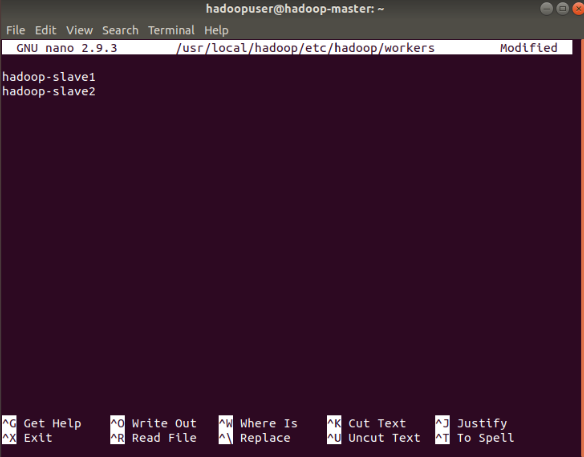
\includegraphics[width=6cm]{32.png}
\caption{\label{}}
\end{figure}
.\\\\
We need to copy the Hadoop Master configurations to the slaves, to do that we use these commands:

\begin{lstlisting}[language=Python, caption= a ]
scp /usr/local/hadoop/etc/hadoop/* hadoop-slave1:/usr/local/hadoop/etc/hadoop//
\end{lstlisting}

\begin{figure}[ht!]
\centering
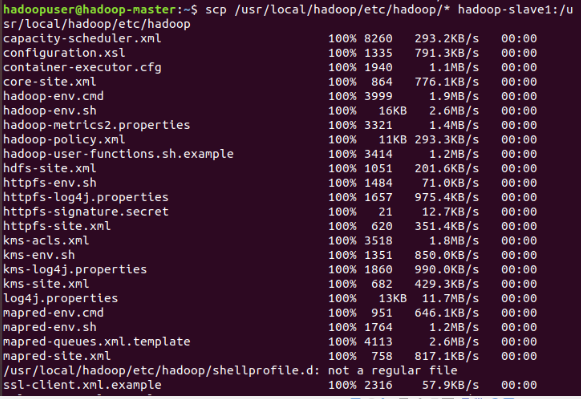
\includegraphics[width=8cm]{33.png}
\caption{\label{}}
\end{figure}

\begin{lstlisting}[language=Python, caption= a ]
scp /usr/local/hadoop/etc/hadoop/* hadoop-slave2:/usr/local/hadoop/etc/hadoop/
\end{lstlisting}

\begin{figure}[ht!]
\centering
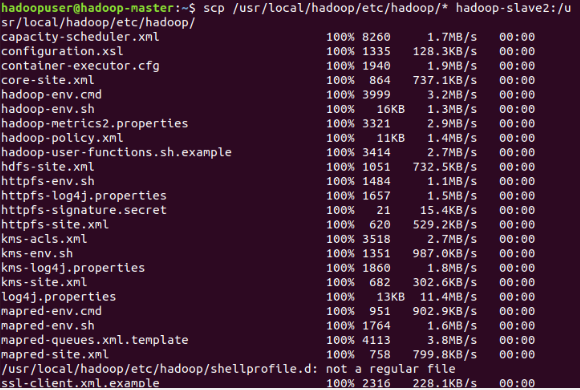
\includegraphics[width=8cm]{34.png}
\caption{\label{}}
\end{figure}

\section{HDFS}

\subsection{format hdfs}
Now we need to format the HDFS file system. Run these commands:

\begin{lstlisting}[language=Python, caption= a ]
source /etc/environment
hdfs namenode -format
\end{lstlisting}

\begin{figure}[ht!]
\centering

\includegraphics[width=8cm]{35.png}
\caption{\label{}}
\end{figure}


\subsection{start hdfs}

Start HDFS with this command:

\begin{lstlisting}[language=Python, caption= a ]
start-dfs.sh
\end{lstlisting}


\begin{figure}[ht!]
\centering
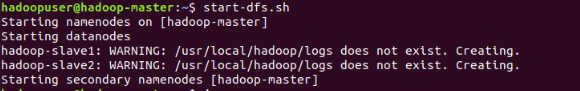
\includegraphics[width=8cm]{36.png}
\caption{\label{}}
\end{figure}


To check if this worked, run the follwing command. This will tell you what resources have been initialized:

\begin{lstlisting}[language=Python, caption= for all nodes ]
jps
\end{lstlisting}


\begin{figure}[ht!]
\centering
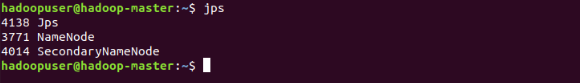
\includegraphics[width=8cm]{37.png}
\caption{\label{}}
\end{figure}


\begin{figure}[ht!]
\centering
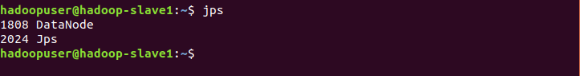
\includegraphics[width=8cm]{38.png}
\caption{\label{}}
\end{figure}


\begin{figure}[ht!]
\centering
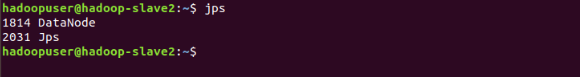
\includegraphics[width=8cm]{39.png}
\caption{\label{}}
\end{figure}


Let’s see if this worked:
Open your browser and type \textbf{hadoop-master:9870}
This is what mine shows, hopefully yours is showing the same thing!\\\\\\\\


\begin{figure}[ht!]
\centering
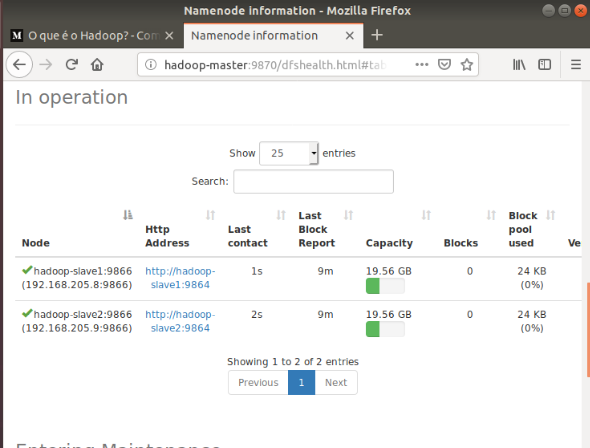
\includegraphics[width=8cm]{40.png}
\caption{\label{}}
\end{figure}


As you can see, both nodes are operational!






\section{Resources}


\url{https://medium.com/@jootorres_11979/how-to-set-up-a-hadoop-3-2-1-multi-node-cluster-on-ubuntu-18-04-2-nodes-567ca44a3b12}

\url{https://www.digitalocean.com/community/tutorials/how-to-install-hadoop-in-stand-alone-mode-on-ubuntu-18-04}

\url{https://archive.apache.org/dist/hadoop/core/hadoop-3.0.3/}

\url{https://data-flair.training/blogs/install-hadoop-on-ubuntu/}



\end{document}

